\chapter{Experiments}\label{chap:experiments}
%\begin{itemize}
%	\item lokale Experimente(?)
%	\item Eindeutige Benennung der Datensätze, auch in plots (vor allem emnist vs mnist!)
%	\item beschreiben, wie ich SVHN und CIFAR10 in tff lade (SqlClientData), als Implementierungsdetails
%	\item durch den Code gehen und schauen ob ich alle Punkte aufgeschrieben habe
%\end{itemize}

% genau auf Experimente und deren Setups eingehen
Ich evaluiere meinen Algorithmus auf drei Datensätzen, MNIST \cite{lecun:1998}, SVHN \cite{netzer:2011} und CIFAR10 \cite{krizhevsky:2009}. Im Vordergrund steht dabei die erreichbare Genauigkeit im Vergleich zu der Nutzung einheitlicher Privacy Budgets. Anders als \textcite{aldaghri:2023} untersuche ich jedoch auch unterschiedliche Verteilungen innerhalb der individualisierten Privacy Budgets. Abgesehen von den Auswirkungen von Differential Privacy auf die Genauigkeiten der Modelle, betrachte ich auch die Verteilung der Daten auf den Clients. Da wie in \autoref{fund-fl} beschrieben auch die Verzerrung der Trainingsdaten Auswirkungen auf die Ergebnisse hat erstelle ich für die Datensätze auch eine gleichverteilte Version.

\begin{figure}[h]
	\centering
	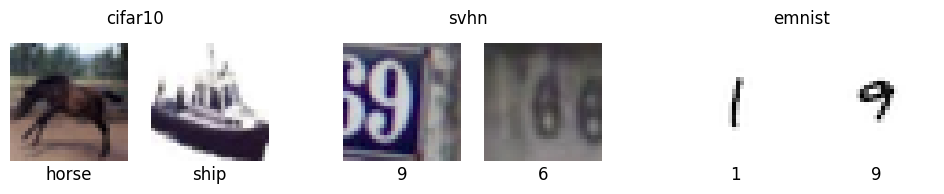
\includegraphics[width=0.9\textwidth]{Bilder/dataset_examples.png}
	\caption{Examples from the three training datasets}
	\label{fig:dataset-examples}
\end{figure}

\section{Environment}
Ich habe den Algorithmus aus \autoref{chap:methods} mit Python in Tensorflow Federated implementiert. Das ist ein auf Tensorflow aufgebautes Framework, das das Federated Training von Neuronalen Netzen, die in Tensorflow definiert werden, relativ einfach gestaltet. Das Framework ist sehr modular aufgebaut und erlaubt es Schritte im Federated Learning, wie zum Beispiel die Aggregation der Updates durch eine andere Aggregation auszutauschen. Abgesehen vom Federated Learning hat das Framework mit Federated Core den Anspruch, eine Basis für verteilte Berechnungen zu sein. Dafür hat es beispielsweise Datentypen so adaptiert, dass sie abgesehen vom eigentlichen Datentypen immer auch die Geräte beinhalten, an denen sie sich befinden. Die High-level Federated Learning API beinhaltet typische Algorithmen wie \texttt{FedAvg} oder \texttt{DP-FedAvg}.

\autoref{alg:boenisch-sample} habe ich so adaptiert, dass statt Opacus die Bibliothek \textit{dp-accounting} genutzt wird. Ich habe mich dazu entschieden, da der Rest meines Environments auf Tensorflow basiert und ich daher PyTorch nicht als weitere Abhängigkeit haben wollte.

Die Berechnungen habe ich auf dem Clara Cluster der Universität Leipzig ausgeführt. Um das Environment aufzusetzen und zu definieren habe ich ein Docker Image definiert, welches Python, CUDA und notwendige Bibliotheken installiert.

\section{Datasets}

\begin{figure}[tb]
	\centering
	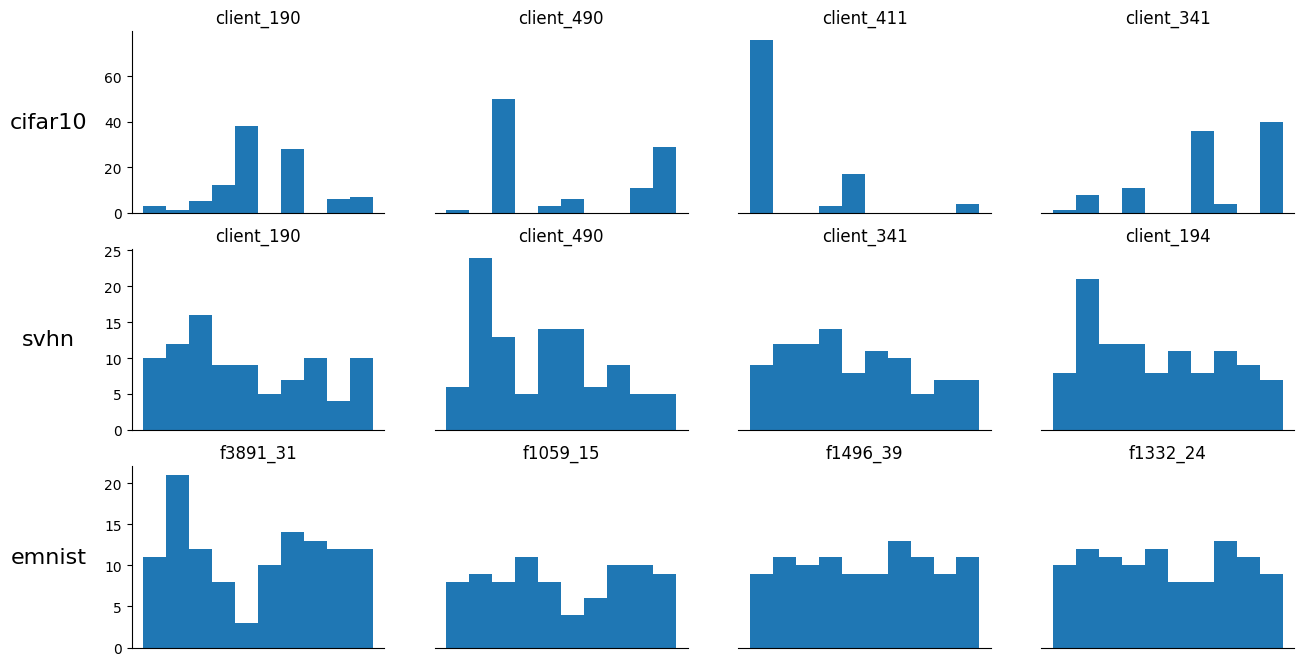
\includegraphics[width=0.9\textwidth]{Bilder/label_distribution.png}
	\caption{Label distribution on exemplary clients from the different datasets}
	\label{fig:label-distribution}
\end{figure}

Der MNIST-Datensatz (Modified National Institute of Standards and Technology) ist ein weit verbreiteter Benchmark im Bereich des maschinellen Lernens, insbesondere für Bildklassifizierungsaufgaben. Er besteht aus 70.000 Graustufenbildern handgeschriebener Ziffern, wobei jedes Bild eine Größe von 28x28 Pixeln hat. Der Datensatz ist in 60.000 Trainingsbilder und 10.000 Testbilder unterteilt, wobei die Ziffern von 0 bis 9 reichen. Jedes Bild ist mit der entsprechenden Ziffer beschriftet, was es zu einem überwachten Lernproblem macht. Aufgrund seiner Einfachheit und Relevanz wird der MNIST-Datensatz häufig zum Testen neuer Algorithmen und Modelle in Aufgaben wie der Ziffernerkennung verwendet.

Tensorflow Federated stellt einen Datensatz bereit, der auf einer erweiterten Version von MNIST basiert. Die Ziffern sind dabei nach ihrem jeweiligen Autor aufgeteilt, was eine realistische Annahme im Federated Learning ist. Die Methodik bei der Aufteilung folgt \textcite{caldas:2018}. So wird ein \textit{Feature Distribution Skew} aus \autoref{fund-fl-data-heterogenity} simuliert. In \autoref{fig:emnist-feature-skew} ist die handgeschriebene Ziffer 8 von verschiedenen Clients zu sehen. Die unterschiedlichen Handschriften sind klar zu erkennen und stellen in diesem Datensatz die Verzerrung der Features dar.

\begin{figure}[tb]
	\centering
	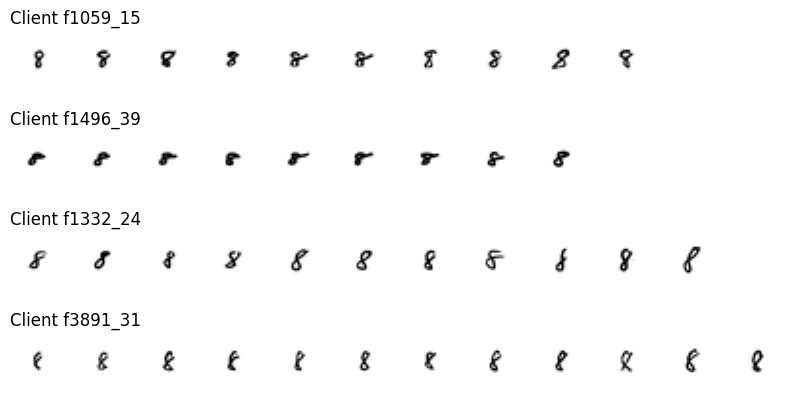
\includegraphics[width=0.8\textwidth]{Bilder/emnist_feature_distribution_skew.png}
	\caption{The digit eight from different clients in MNIST showing the different handwritings}
	\label{fig:emnist-feature-skew}
\end{figure}

\begin{figure}[tb]
	\centering
	\begin{subfigure}{0.3\textwidth}
		\centering
		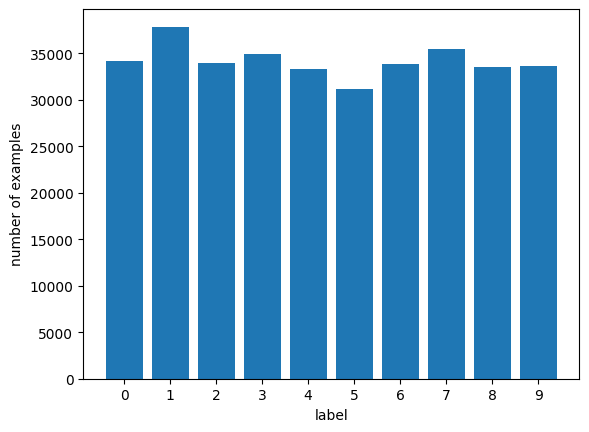
\includegraphics[width=\textwidth]{Bilder/emnist_label_distribution.png}
		\caption{EMNIST}
	\end{subfigure}
	\begin{subfigure}{0.3\textwidth}
		\centering
		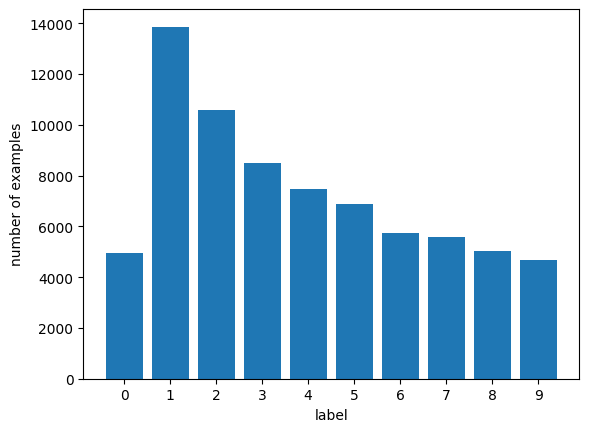
\includegraphics[width=\textwidth]{Bilder/svhn_label_distribution.png}
		\caption{SVHN}
	\end{subfigure}
	\begin{subfigure}{0.3\textwidth}
		\centering
		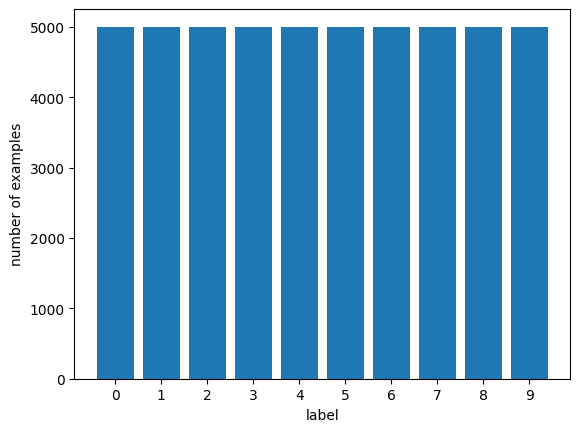
\includegraphics[width=\textwidth]{Bilder/cifar_label_distribution.png}
		\caption{CIFAR-10}
	\end{subfigure}
	\caption{Distribution of labels in the training datasets among all clients}
	\label{fig:label-distribution-all}
\end{figure}

Der SVHN-Datensatz (Street View House Numbers) ist ein weiterer bekannter Datensatz im Bereich des maschinellen Lernens, der häufig für Bildklassifizierungsaufgaben verwendet wird, speziell zur Erkennung von Ziffern. Er besteht aus über 600.000 farbigen Bildern von Hausnummern, die aus Google Street View-Aufnahmen extrahiert wurden. Jedes Bild enthält eine Ziffer (0-9) und ist in verschiedene Datensätze für Training und Testen unterteilt. Im Gegensatz zum MNIST-Datensatz, der handgeschriebene Ziffern zeigt, stellt SVHN ein anspruchsvolleres Problem dar, da die Ziffern aus der realen Welt stammen und häufig von komplexen Hintergründen, Beleuchtungsschwankungen und verschiedenen Schriftarten beeinflusst werden. SVHN ist daher ein wertvoller Datensatz zur Entwicklung und Evaluierung von Algorithmen, die unter realen Bedingungen gut funktionieren.

Es gibt keine Version dieses Datensatzes innerhalb von Tensorflow Federated, daher habe ich die Trainingsdaten zufällig auf eine Anzahl von Clients verteilt. Um zu verhindern, dass Clients jedes Mal andere Daten zugewiesen werden, habe ich den erstellten Datensatz in dem Tensorflow Federated \texttt{SqlClientData}-Format\footnote{\url{https://www.tensorflow.org/federated/api_docs/python/tff/simulation/datasets/SqlClientData} (accessed 28-11-2024)} gespeichert.

Der CIFAR-10-Datensatz (Canadian Institute For Advanced Research) ist ein bekannter Benchmark-Datensatz im Bereich des maschinellen Lernens und der Bildklassifikation. Er enthält 60.000 farbige Bilder mit einer Größe von 32x32 Pixeln, die in 10 verschiedene Klassen unterteilt sind: Flugzeuge, Autos, Vögel, Katzen, Hirsche, Hunde, Frösche, Pferde, Schiffe und Lastwagen. Jede Klasse ist mit 6.000 Bildern repräsentiert, und der Datensatz ist in 50.000 Trainingsbilder und 10.000 Testbilder aufgeteilt. CIFAR-10 stellt eine größere Herausforderung als einfachere Datensätze wie MNIST dar, da die Bilder vielfältigere und komplexere Objekte aus der realen Welt enthalten. 

Tensorflow Federated beinhaltet zwar keine Version des CIFAR-10 Datensatzes, allerdings gibt es den CIFAR-100-Datensatz \cite{krizhevsky:2009}. Jedoch ist dieser noch komplexer, daher habe ich mich entschlossen den CIFAR-10 Datensatz so aufzubereiten, wie es beim Tensorflow Federated CIFAR-100 Datensatz gemacht wurde. 

Dort wird für jeden Client ein Vektor aus der Dirichlet-Verteilung gezogen, welcher für jede Klasse die Wahrscheinlichkeit repräsentiert, ein Trainingsbeispiel aus der jeweiligen Klasse zu ziehen. Dementsprechend zieht jeder Client Beispiele aus dem Datensatz. Wenn eine Klasse keine weiteren Daten enthält, wird der Zahlenvektor für jeden Client neu gezogen, allerdings nur mit den Klassen, die noch nicht aufgebraucht sind. Am Ende erhält man so Clients, bei denen die Klassen je nach Client unterschiedlich stark vertreten sind und es wird ein \textit{Label Distribution Skew} aus \autoref{fund-fl-data-heterogenity} abgebildet. Der Effekt ist in \autoref{fig:label-distribution} zu sehen. Die Verteilung der Klassen bei den CIFAR-10 Clients ist sehr viel unregelmäßiger als die der anderen Datensätze und hat viele Lücken.

\autoref{fig:label-distribution-all} zeigt die Verteilung der Labels in den gesamten Trainingsdaten. Es ist auffällig, dass es in SVHN deutlich mehr kleinere Ziffern gibt als größere, mit Ausnahme der $0$. Allerdings lässt sich das womöglich dadurch erklären, dass Hausnummern in der Regel aufsteigend vorliegen und es daher für jede Ziffer $9$ auch $1$ bis $8$ gegeben haben muss. Diese ungleiche Verteilung wirkt sich, wie in \autoref{fig:label-distribution} zu sehen ist, auch auf die Menge der Trainingsbeispiele auf den Clients aus.

\section{IID versions of the datasets}\label{sec:iid-dataset-creation}
Für MNIST und CIFAR-10 erstelle ich abgesehen von den oben genannten Datensätzen noch eine Version, bei der die Daten zufällig auf den Clients verteilt werden. Der Grund dafür ist, dass \texttt{FedAvg}, auf dem mein Algorithmus basiert, Schwierigkeiten mit Verzerrungen in den Trainingsdaten hat. Diese Versionen sollen also vor allem als eine Baseline sein und zur Vergleichbarkeit meiner Ergebnissen beitragen.

\textit{Tensorflow Federated} stellt für die Erstellung gleichverteilter Datensätze eine Funktion bereit.\footnote{\url{https://www.tensorflow.org/federated/api_docs/python/tff/simulation/datasets/build_synthethic_iid_datasets}, (accessed 07-11-2024)} Diese erstellt einen \texttt{Iterator}, bei dem in jeder Iteration zufällig aus allen Trainingsdaten gezogen wird. Damit gibt es jedoch keine Zuweisung mehr von den Daten zu den Clients, das heißt wenn ein Client gezogen wird, werden seine Trainingsdaten dynamisch zusammengesetzt.

Ich wollte in meinem Fall gerne eine Beziehung der Clients zu den Daten beibehalten, das heißt wenn in meinem Fall der gleiche Client in verschiedenen Runden gezogen wird, trainiert er auch auf den gleichen Daten.

Dazu habe ich eine Funktion geschrieben, die einen Datensatz als Eingabe bekommt und dann die Datenpunkte zufällig den Clients zuweist. Diese Funktion liefert dann einen Datensatz zurück in dem Clients feste Datenpunkte zugewiesen sind.

\section{Model Architecture}
Die Datensätze, auf denen ich meinen Algorithmus auswerte sind für Bildklassifizierungen gemacht. Daher verwende ich in meinen Experimenten ein einfaches Convolutional Neural Network. Das Neuronale Netz ist für alle Datensätze das gleiche, lediglich die \texttt{input\_shape} passe ich den jeweiligen Daten an. Außerdem gibt es einen Rescaling Layer, der die Pixel auf das Intervall $[0;1]$ normalisiert. Bei MNIST ist das nicht nötig, da bereits alle Werte zwischen $0$ und $1$ liegen.

Das Neuronale Netz selbst ist sehr klein und enthält nur $21578$ trainierbare Parameter. Ich habe mich dafür entschieden, das Training damit durchzuführen, da größere Modelle einen erheblichen Mehraufwand beim Training bedeuten, weil im Trainingsprozess viele Clients simuliert werden müssen. Bereits bei auf Effizienz ausgerichteten Modellen wie \textit{MobileNet} \cite{howard:2017} und \textit{EfficientNet} \cite{tan:2019} war ein zügiges Training nicht mehr möglich.

Die Schichten des Modells bestehen aus Convolutional, MaxPooling und Dropout Layern. Darüber hinaus gibt es am Ende zwei Linear Layers für die Klassifikation.

\begin{figure}[tb]
	\centering
	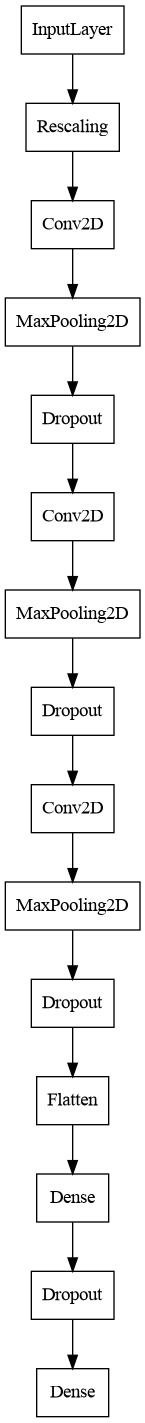
\includegraphics[height=0.6\textheight]{Bilder/model_architecture.png}
	\caption{Architecture of the model used for the classification tasks}
	\label{fig:model-architecture}
\end{figure}

Um das Training einfach zu halten habe ich auf weitere Vorverarbeitungsschritte der Bilder verzichtet. Ich führe auch keine Augmentation der Trainingsdaten durch, zum Beispiel durch zufälliges drehen oder zuschneiden der Bilder.

Durch lokale Experimente auf zentralen Trainingsdaten habe ich überprüft, dass mein Modell auf allen Datensätzen in der Lage ist zu lernen. Daher ist das Modell für mein Ziel ausreichend, nämlich meinen Trainingsalgorithmus zu testen und Aussagen über die Auswirkungen verschiedener Parameter zu treffen.

\section{Privacy Setups}
Ich führe die Experimente jeweils mit insgesamt fünf Privacy-Niveaus durch. Im folgenden werde ich mich mit den Namen \texttt{no-dp}, \texttt{relaxed-dp}, \texttt{relaxed-idp}, \texttt{strict-idp} und \texttt{strict-dp} auf diese beziehen. In dieser Reihenfolge haben sie ansteigende Anforderungen an die Differential Privacy. \autoref{tab:privacy-niveau-distribution} zeigt die Verteilung der Privacy Budgets für jedes der Setups. \texttt{strict-idp} und \texttt{relaxed-idp} sind die beiden Setups, die mit individualisierten Privacy Budgets arbeiten. Die anderen nutzen entweder homogene Budgets oder gar keine und dienen zum Vergleich mit meinen Ergebnissen. Die Erwartung ist, dass \texttt{no-dp} und \texttt{relaxed-dp} besser abschneiden, als \texttt{relaxed-idp} und \texttt{strict-idp}, während \texttt{strict-dp} die größten Abstriche bei der Nützlichkeit erwarten lässt.

\begin{table}[tb]
	\centering
	\begin{tabular}{|c|c|c|c|}
		\hline
		Level & $\epsilon_1$ & $\epsilon_2$ & $\epsilon_3$ \\
		\hline
		\texttt{no-dp} & - & - & - \\
		\texttt{relaxed-dp} & - & - & $100\%$ \\
		\texttt{relaxed-idp} & $34\%$ & $43\%$ & $23\%$ \\
		\texttt{strict-idp} & $54\%$ & $37\%$ & $9\%$ \\
		\texttt{strict-dp} & $100\%$ & - & - \\
		\hline
	\end{tabular}
	\caption{The distribution of Privacy Budgets in the different Privacy Setups with $\epsilon_1$ being the smallest, $\epsilon_2$ the intermediate and $\epsilon_3$ the largest Privacy Budget}
	\label{tab:privacy-niveau-distribution}
\end{table}

Für jeden Datensatz definiere ich drei Privacy-Budgets jeweils für Clients die niedrige, mittlere und hohe Anforderungen an ihre Privatheit haben. Ich musste in meinen Experimenten feststellen, dass einheitliche Budgets über alle Datensätze nicht funktionieren, weil die Modelle dann bei SVHN und CIFAR-10 nicht konvergieren. Das unterstreicht noch einmal unterschiedlichen Schwierigkeitsgrade zwischen den Datensätzen.

\begin{table}[tb]
	\centering
	\begin{tabular}{|c|c|c|c|}
		\hline
		Dataset & $\epsilon_1$ & $\epsilon_2$ & $\epsilon_3$ \\
		\hline
		MNIST & $1.0$ & $2.0$ & $3.0$ \\
		SVHN & $15.0$ & $25.0$ & $40.0$ \\
		CIFAR10 & $15.0$ & $25.0$ & $40.0$ \\
		\hline
	\end{tabular}
	\caption{The Privacy Budgets for each dataset}
	\label{tab:privacy-budgets-per-dataset}
\end{table}

Die Annahmen, dass es drei Gruppen mit unterschiedlichen Anforderungen an die Privatheit gibt und auch die Verteilungen dieser Gruppen innerhalb der Clients folgt \textcite{boenisch:2023} und ist durch empirische Studien gedeckt \cite{jensen:2005, acquisti:2005}. Eine Übersicht der Budgets auf den Datensätzen steht in \autoref{tab:privacy-budgets-per-dataset}.

%\begin{table}[tb]
%	\centering
%	\begin{tabular}{|c|c|c|c|c|c|c|c|}
%		\hline
%		\multirow{2}{4em}{Dataset} & \multicolumn{3}{|c|}{Whole Dataset} & \multicolumn{4}{|c|}{Per Client} \\
%		\cline{2-8}
%		& \#examples & \#classes & \#clients & $\diameter$examples & $\sigma$examples & $\diameter$classes & $\sigma$classes \\
%		\hline
%		MNIST & 341873 & 10 & 3383 & 101.05 & 14.72 & 9.99 & 0.14 \\
%		SVHN & 26032 & 10 & 725 & 35.91 & 5.89 & 9.45 & 0.76 \\
%		CIFAR-100 & 50000 & 20 & 500 & 100.0 & 0.0 & 6.53 & 1.99 \\
%		\hline
%	\end{tabular}
%	\caption{Some statistics of the different datasets for (1) the whole dataset and (2) the individual clients}
%	\label{tab:dataset-statistics}
%\end{table}


